
{\Large \textbf{Experience}}\\[-0.4cm]
\makebox[\linewidth]{\rule{1.0\textwidth}{0.4pt}} \\
\vspace{0cm}
%%%%%%%%%%%%%%%%%%%%%%%%%%%%%%

\begin{center}
    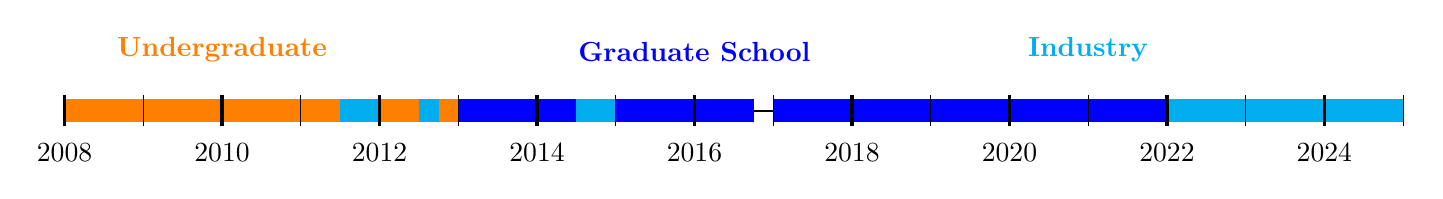
\begin{tikzpicture}
        % Labels above timeline
        \node[above, orange] at (2,0.5) {\textbf{Undergraduate}};
        \node[above, blue] at (8,0.5) {\textbf{Graduate School}};
        \node[above, cyan] at (13,0.5) {\textbf{Industry}};
        
        % Full timeline base (thin gray for reference)
        \draw[thick, black] (0,0) -- (17,0); 
        % Graduate School section (Blue, thicker)
        \draw[line width=3mm, orange] (0,0) -- (5,0);
        \draw[line width=3mm, blue] (5,0) -- (8.75,0);
        \draw[line width=3mm, blue] (9,0) -- (14,0);
        % Industry section (Green, thicker)
        \draw[line width=3mm, cyan] (3.5,0) -- (4,0);
        \draw[line width=3mm, cyan] (4.5,0) -- (4.75,0);
        \draw[line width=3mm, cyan] (6.5,0) -- (7,0);
        \draw[line width=3mm, cyan] (14,0) -- (17,0);
        % Add year markers
        \foreach \x/\year in {0/2008, 2/2010, 4/2012, 6/2014, 8/2016, 10/2018, 12/2020, 14/2022, 16/2024} {
            \draw[very thick] (\x,0.2) -- (\x,-0.2);
            \node[below] at (\x,-0.3) {\year};
        }
        \foreach \x/\year in {1/2009, 3/2011, 5/2013, 7/2015, 9/2017, 11/2019, 13/2021, 15/2023, 17/2025} {
            \draw[line width=0.1mm] (\x,0.2) -- (\x,-0.2);
            {\year};
        }
    \end{tikzpicture}
\end{center}


% \begin{center}
%     \begin{tikzpicture}
%         % Full timeline base (thin gray for reference)
%         \draw[thick, black] (-1,0) -- (12,0); 
%         % Graduate School section (Blue, thicker)
%         \draw[line width=3mm, blue] (0,0) -- (9,0);
%         % Industry section (Green, thicker)
%         \draw[line width=3mm, cyan] (9,0) -- (12,0);
%         % Add year markers
%         \foreach \x/\year in {0/2013, 2/2015, 4/2017, 6/2019, 8/2021, 10/2023, 12/2025} {
%             \draw[very thick] (\x,0.2) -- (\x,-0.2);
%             \node[below] at (\x,-0.3) {\year};
%         }
%         \foreach \x/\year in {-1/2012, 1/2014, 3/2016, 5/2018, 7/2020, 9/2022, 11/2024} {
%             \draw[line width=0.1mm] (\x,0.2) -- (\x,-0.2);
%             {\year};
%         }
%         % Labels above timeline
%         \node[above, blue] at (4,0.6) {\textbf{Graduate School}};
%         \node[above, cyan] at (10,0.6) {\textbf{Industry}};

%     \end{tikzpicture}
% \end{center}

















\textbf{\href{https://nutrienagsolutions.com/}{{\color{black}Nutrien Ag Solutions}}} 
    \textbf{\href{https://waypointanalytical.com/}{{\color{black} (Waypoint Analytical)}}} | Soil Biome | Champaign, Illinois  \hfill Jan 2022 – \textit{present} \\
    \tab \textbf{Bioinformatics Senior Computational Scientist} \\
    \begin{addmargin}[1cm]{2cm}
    \begin{itemize}[left=-0.2cm, itemsep=-0.15cm]
        \item Developmed end-to-end NGS data pipelines for metagenomic samples.
        \item Built and maintained NextFlow workflows in cloud-computing environments on AWS and GCP.
        \item Developed custom software in \CC\ for lab processing of qPCR data.
        \item Developed packages in both R and python for advanced microbiome data analyses.
        \item Collect and Maintained databases for both lab and computational teams.
        \item Constructed soil-biome report generation platform.
        \item Implemented models and algorithms for product-placement using microbiome metrics.
        \item Implemented RAG and GenAI systems for custom chatbot apps.
        \item Implemented gRPC server and protocols for API data system for biome team.
        \item Project lead for development of metagenomic results discovery database.
        \item Developed analyses and presentations for stakeholders.
        \item Mentored junior colleagues and summer interns.
    \end{itemize}
    \end{addmargin} 

% \textbf{Part-time Research Associate} \hfill May 2023 – May 2024 \\
%     \tab \textbf{Iowa State University} | \href{https://faculty.sites.iastate.edu/rpwise/}{{\color{black}Wise Laboratory}} | Ames, Iowa  \\
%     \begin{addmargin}[1cm]{2cm}
%     \begin{itemize}[left=-0.2cm, itemsep=-0.15cm]
%         \item Containerized lab software for improved usability.
%         \item Genomics analysis to support other lab members.
%         \item Processed NGS DNA and RNA-seq data.
%     \end{itemize}
%     \end{addmargin}

\textbf{Iowa State University} | \href{http://www.germslab.org/}{{\color{black}GERMS Laboratory}} | Ames, Iowa \hfill Jan 2017 - Dec 2021  \\
    \tab \textbf{Graduate Research Assistant - Ph.D.} 
    \begin{addmargin}[1cm]{2cm}
    \begin{itemize}[left=-0.2cm, itemsep=-0.15cm]
        \item Developed pipeline for processing 16S sequencing.
        \item Authored R-packages for microbiome data analysis.
        \item Published research on antibiotic-resistance gene dispersal in environmental systems.
        \item Conducted research on harmful algal bloom biome-community and predictors.
        \item Published research evaluating large-scale marker detection for microbiome genes.
        \item Mentored junior lab members.
        \item Instructor for Data \& Software Carpentries workshops.
    \end{itemize}
    \end{addmargin}

\textbf{University of Wisconsin - Madison} | Potato Genetics Lab | Madison, Wisconsin \hfill Jun 2015 - Sep 2016 \\
    \tab \textbf{Graduate Research Assistant - Ph.D.} \\
    \begin{addmargin}[1cm]{2cm}
    \begin{itemize}[left=-0.2cm, itemsep=-0.15cm]
        \item Developed pipeline for NGS data and SNP-calling for autotetraploid crops.
        \item Authored R-packages for ML methods for autotetraploid genotyping.
    \end{itemize}
    \end{addmargin}

\textbf{USDA-ARS} | Arid-Land Agricultural Research Center | Maricopa, Arizona \hfill Jun 2014 - Dec 2014 \\
    \tab \textbf{Biological Science Technician - Internship} \\
    \begin{addmargin}[1cm]{2cm}
    \begin{itemize}[left=-0.2cm, itemsep=-0.15cm]
        \item Evaluated use of image-based high-throughput phenotyping platforms.
    \end{itemize}
    \end{addmargin}
        
\textbf{Texas A\&M University} | Maize Genetics Lab | College Station, Texas \hfill Jan 2013 - May 2015 \\
    \tab \textbf{Graduate Research Assistant - M.S.} \\
    \begin{addmargin}[1cm]{2cm}
    \begin{itemize}[left=-0.2cm, itemsep=-0.15cm]
        \item Published research characterizing markers of Texas maize germplasm.
    \end{itemize}
    \end{addmargin}

\textbf{Monsanto Company} | Huxley Research Station | Huxley, Iowa \hfill May 2012 - Sep 2012 \\
    \tab \textbf{Maize Breeding Intern} \\
    
\textbf{DuPont Pioneer} | Willmar Research Station | Willmar, Minnesota \hfill Jun 2011 - Dec 2011 \\
    \tab \textbf{Maize Product Trait Development Intern – 6 month} \\
    
% \textbf{Undergraduate Research Assistant} \hfill 2010 - 2011 \\
%     \tab United States Department of Agriculture - Ames, Iowa \\
%     \tab Soybean Genomics Laboratory - Graham Lab 	\\
